In this section, we discuss the performance of \pred\ (\gt) when there is no latent structure in the data, that is the $K$-armed bandits. Then we compare the performance of \pred\ (\gt) against \dpt.

\textbf{Baselines:} In the K-armed bandits We implement the same baselines discussed in \Cref{sec:short-horizon}. The baselines are \pred, \predt, \dptg, \ad, \ts, and \linucb. In the linear and non-linear setting, we compare against \dpt\ instead of \dptg. 

\textbf{Settings:} In the K-armed bandit setting we consider $d=6$, and the arms as canonical vectors $\be_1, \be_2, \ldots, \be_6$. For each task $m$, we choose the hidden parameter $\btheta_{m,*}$ similar to the linear bandit setting discussed in \Cref{sec:linear}. Note that this results in a K-armed bandit setting. For the linear and non-linear setting comparison, we use the same setting as \Cref{sec:linear}, and \ref{sec:short-horizon}.

\textbf{Outcomes:} We first discuss the main outcomes from our experimental results in K-armed bandits and then in comparison against \dpt\ in linear and non-linear settings.


\begin{tcolorbox}
\customfinding \pred\ (\gt) matches the performance of the demonstrator when there is no structure (K-armed bandits). \pred\ (\gt) performs close to \dpt\ in the linear and non-linear setting showing the usefulness of learning the reward structure.
\end{tcolorbox}


\begin{figure}[!hbt]
\centering
\begin{subfigure}[b]{0.3\textwidth}
   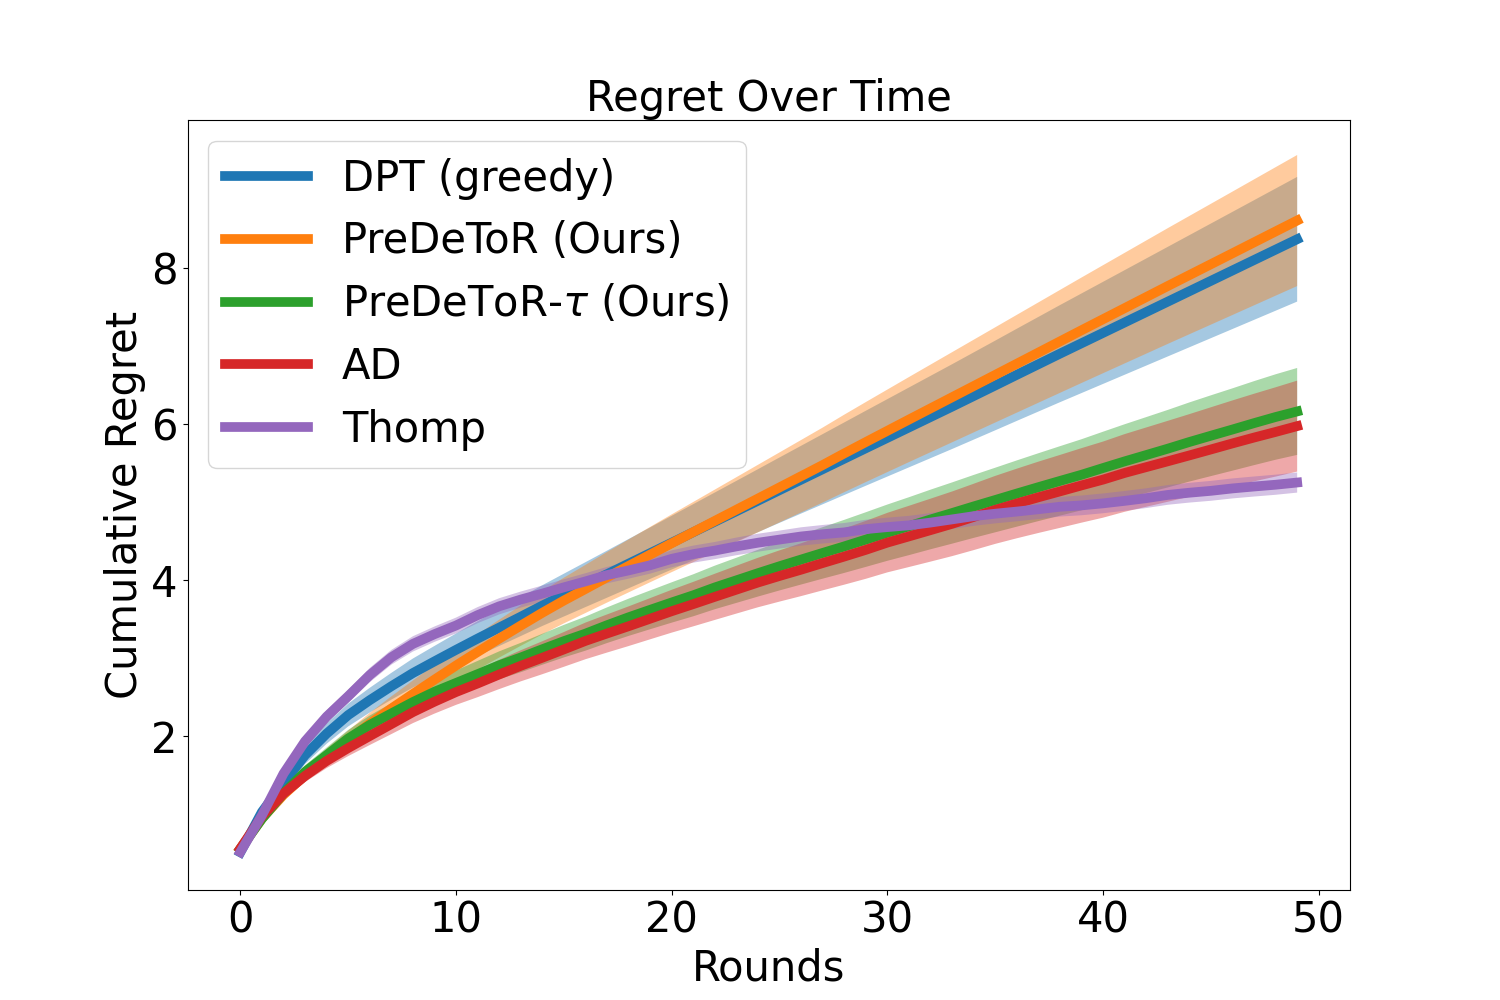
\includegraphics[scale=0.13]{img/Neurips/k_arms_dpt/k_arms_lr0.00015_do0_embd32_layer4_head4_envs200021_hists1_samples1_var0.3_cov0.0_H50_d5_lind5_seed1_testcov0.0_hor50.pkl.png}
   \caption{K-armed Bandit}
   \label{fig:dpt-1}
\end{subfigure}%
\begin{subfigure}[b]{0.3\textwidth}
   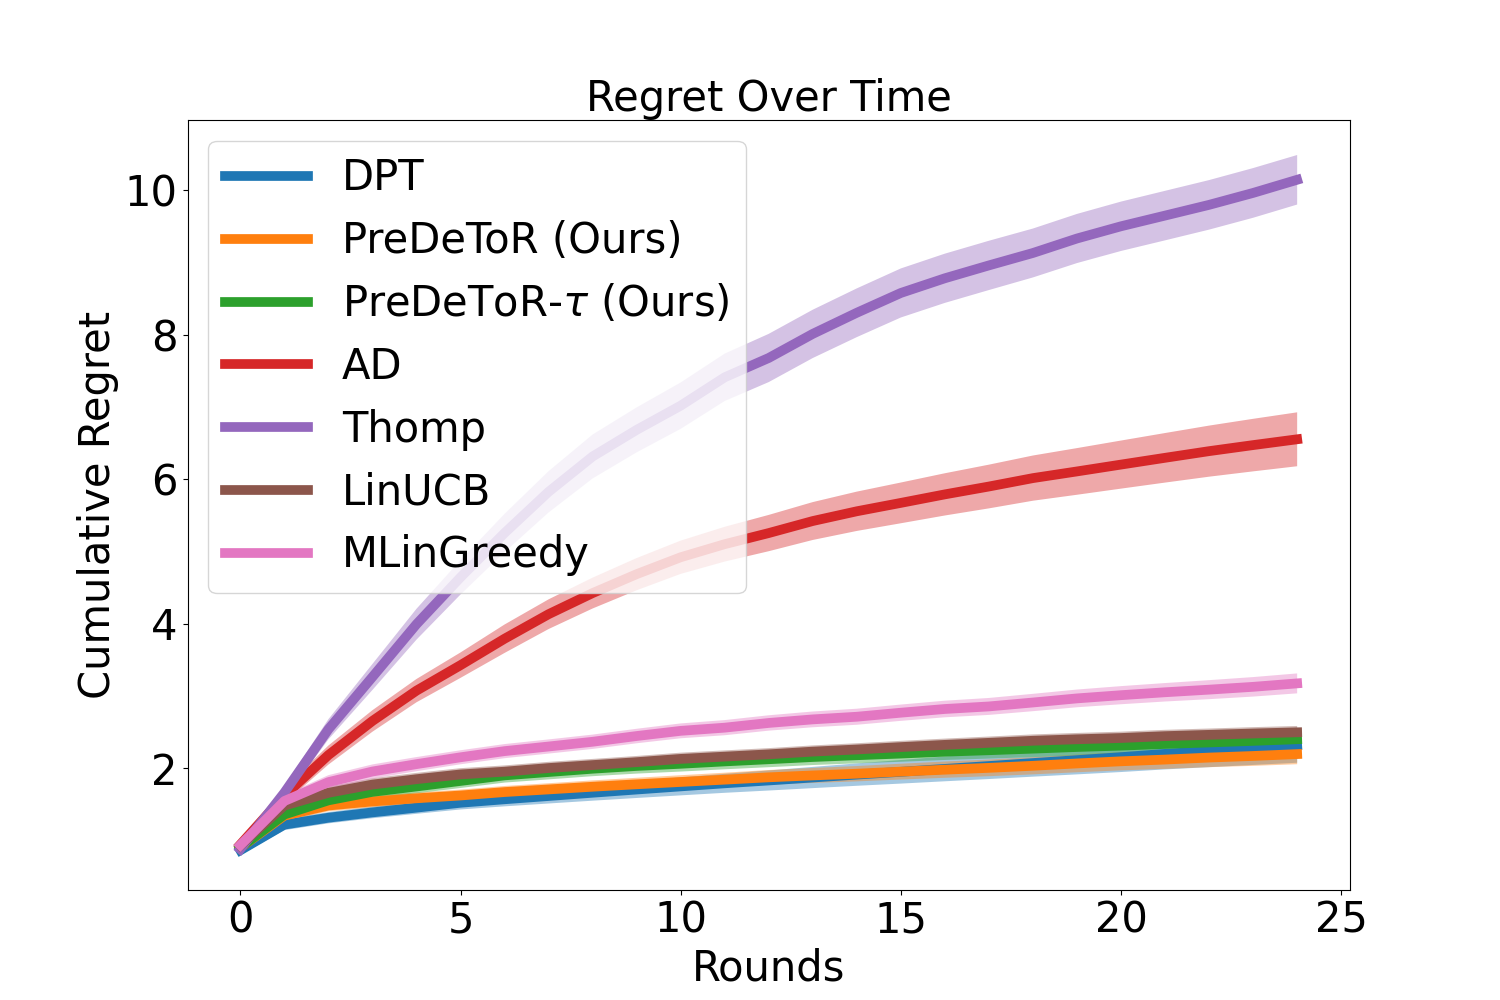
\includegraphics[scale=0.13]{img/Neurips/k_arms_dpt/dpt_lr0.00015_do0_embd32_layer4_head4_envs100067_hists1_samples1_var0.3_cov0.0_H25_d10_lind2_seed1_testcov0.0_hor25.pkl.png}
   \caption{Comparison against \dpt\ in linear setting}
   \label{fig:dpt-2}
\end{subfigure}%
\begin{subfigure}[b]{0.3\textwidth}
   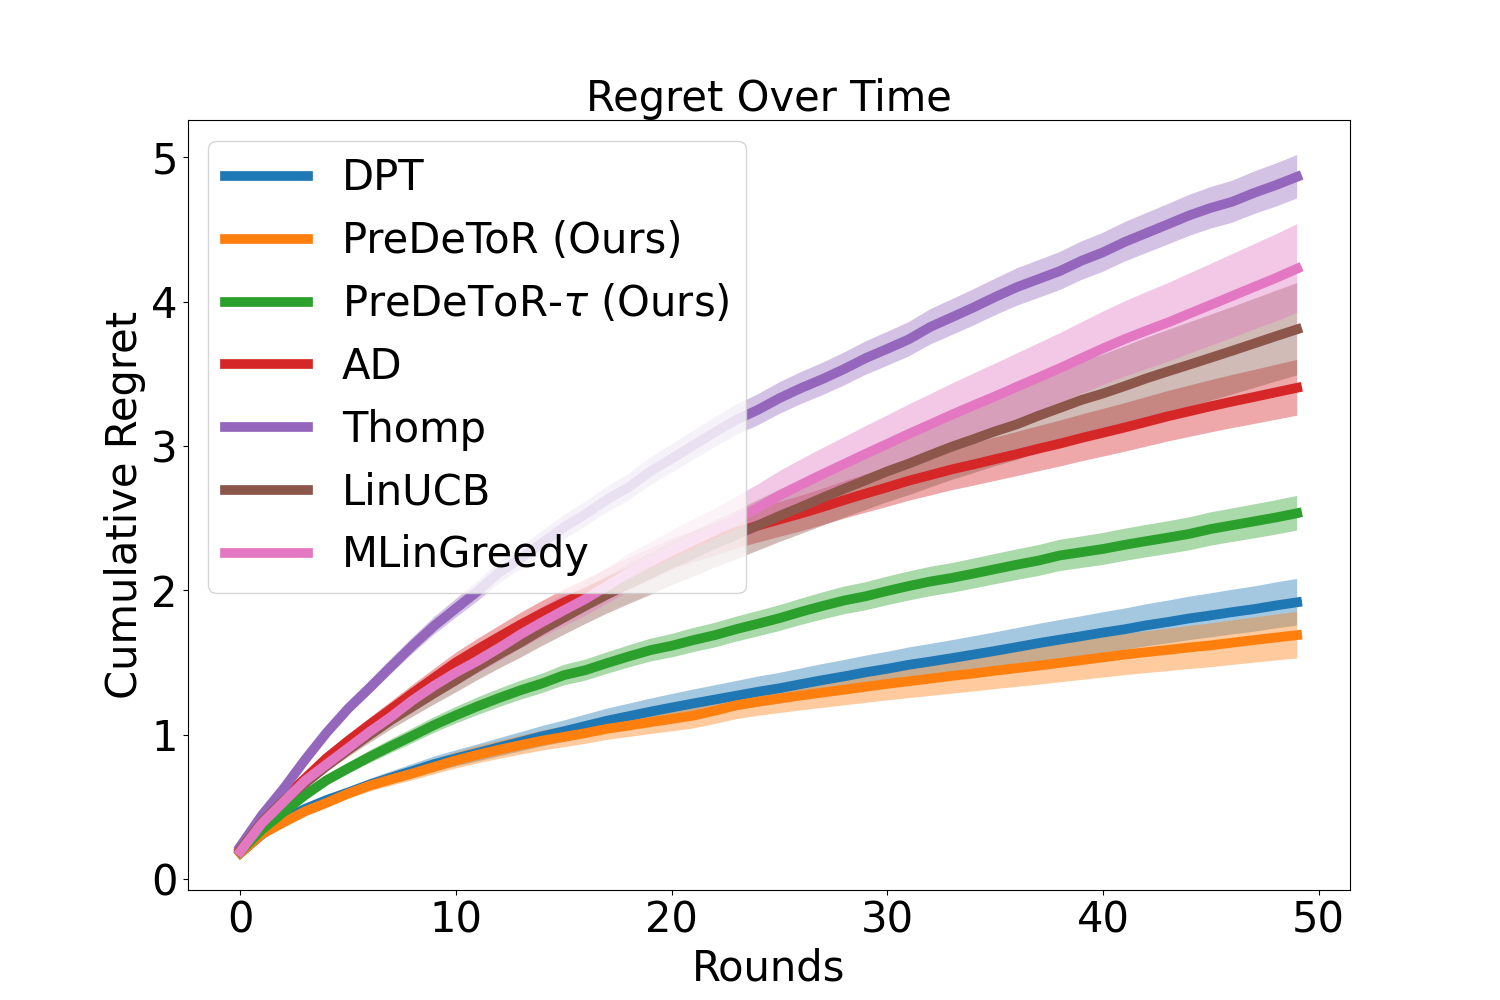
\includegraphics[scale=0.13]{img/Neurips/k_arms_dpt/dpt_nl_lr0.00015_do0_embd32_layer4_head4_envs100467_hists1_samples1_var0.3_cov0.0_H50_d6_lind2_seed1_testcov0.0_hor50.pkl.png}
   \caption{Comparison against \dpt\ in non-linear setting}
   \label{fig:dpt-3}
\end{subfigure}
\vspace*{-1em}
\caption{Experiment with k-armed bandits and \dpt\ (original). The y-axis shows the cumulative regret.}
\label{fig:expt-k-arms-dpt}
\end{figure}


\textbf{Experimental Result:} We observe these outcomes in \Cref{fig:expt-k-arms-dpt}. In \Cref{fig:dpt-1} the demonstrator $\pi^w$ is the \ts\ algorithm. \textit{Note that there is no structure across arms now, and sampling one arm gives no information about other arms in a task.} We observe that \predt\ performs similarly to the demonstrator \ts, and also shows that incorporating exploration is a sound technique. Also, \ad\ performs similarly to the demonstrator \ts. Both \dptg\ and \pred\ fail to learn the latent structure across the tasks and therefore do not learn any exploration strategy. 


In \Cref{fig:dpt-2} we show the linear bandit setting discussed in \Cref{sec:addl-expt}. We observe that \pred\ (\gt) matches the performance of \dpt, and \linucb. Note that \dpt\ has access to the optimal action per task, and \linucb\ is the optimal oracle algorithm that leverages the structure information. 

%
In \Cref{fig:dpt-3} we show the non-linear bandit setting discussed in \Cref{sec:addl-expt}. 
%
Again we observe that \pred\ (\gt) matches the performance of \dpt\ and has lower cumulative regret than \ad\ and \linucb\ which fails to perform well in this non-linear setting due to its algorithmic design. 

